
We have
\begin{align}
    \myvec{2&3}\vec{x}=k \label{aug/2/2/eq.1}
\end{align}
where,
\begin{align}
    \vec{x}=\myvec{x\\y}
\end{align}
Let \begin{align}
    \vec{A}=\myvec{2\\1}
\end{align}
be the solution of \eqref{aug/2/2/eq.1}.
Substituting $\vec{A}$ in \eqref{aug/2/2/eq.1}, we get,
\begin{align}
 k &=7
\end{align}
See Fig. \ref{aug/2/2/Fig 1.1}.
\begin{figure}[h]
\centering
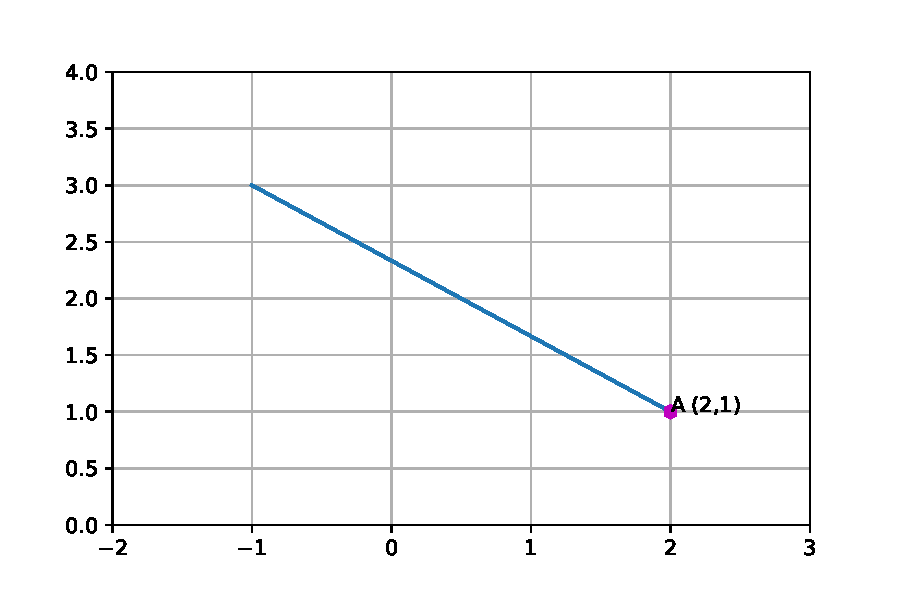
\includegraphics[width=\columnwidth]{solutions/aug/2/2/Figures/line.pdf}
\label{aug/2/2/Fig 1.1}
\caption{}
\end{figure}
